\documentclass[bachelor, och, labwork]{shiza}
% параметр - тип обучения - одно из значений:
%    spec     - специальность
%    bachelor - бакалавриат (по умолчанию)
%    master   - магистратура
% параметр - форма обучения - одно из значений:
%    och   - очное (по умолчанию)
%    zaoch - заочное
% параметр - тип работы - одно из значений:
%    referat    - реферат
%    coursework - курсовая работа (по умолчанию)
%    diploma    - дипломная работа
%    pract      - отчет по практике
% параметр - включение шрифта
%    times    - включение шрифта Times New Roman (если установлен)
%               по умолчанию выключен
\usepackage{subfigure}
\usepackage{tikz,pgfplots}
\pgfplotsset{compat=1.5}
\usepackage{float}

%\usepackage{titlesec}
\setcounter{secnumdepth}{4}
%\titleformat{\paragraph}
%{\normalfont\normalsize}{\theparagraph}{1em}{}
%\titlespacing*{\paragraph}
%{35.5pt}{3.25ex plus 1ex minus .2ex}{1.5ex plus .2ex}

\titleformat{\paragraph}[block]
{\hspace{1.25cm}\normalfont}
{\theparagraph}{1ex}{}
\titlespacing{\paragraph}
{0cm}{2ex plus 1ex minus .2ex}{.4ex plus.2ex}

% --------------------------------------------------------------------------%


\usepackage[T2A]{fontenc}
\usepackage[utf8]{inputenc}
\usepackage{graphicx}
\graphicspath{ {./images/} }
\usepackage{tempora}

\usepackage[sort,compress]{cite}
\usepackage{amsmath}
\usepackage{amssymb}
\usepackage{amsthm}
\usepackage{fancyvrb}
\usepackage{listings}
\usepackage{listingsutf8}
\usepackage{longtable}
\usepackage{array}
\usepackage[english,russian]{babel}

% \usepackage[colorlinks=true]{hyperref}
\usepackage{url}

\usepackage{underscore}
\usepackage{setspace}
\usepackage{indentfirst} 
\usepackage{mathtools}
\usepackage{amsfonts}
\usepackage{enumitem}
\usepackage{tikz}

\newcommand{\eqdef}{\stackrel {\rm def}{=}}
\newcommand{\specialcell}[2][c]{%
\begin{tabular}[#1]{@{}c@{}}#2\end{tabular}}

\renewcommand\theFancyVerbLine{\small\arabic{FancyVerbLine}}

\newtheorem{lem}{Лемма}

\begin{document}

% Кафедра (в родительном падеже)
\chair{}

% Тема работы
\title{IP АДРЕСАЦИЯ КЛАССИЧЕСКИХ СЕТЕЙ}

% Курс
\course{2}

% Группа
\group{231}

% Факультет (в родительном падеже) (по умолчанию "факультета КНиИТ")
\department{факультета КНиИТ}

% Специальность/направление код - наименование
%\napravlenie{09.03.04 "--- Программная инженерия}
%\napravlenie{010500 "--- Математическое обеспечение и администрирование информационных систем}
%\napravlenie{230100 "--- Информатика и вычислительная техника}
%\napravlenie{231000 "--- Программная инженерия}
\napravlenie{100501 "--- Компьютерная безопасность}

% Для студентки. Для работы студента следующая команда не нужна.
% \studenttitle{Студентки}

% Фамилия, имя, отчество в родительном падеже
\author{Окунькова Сергея Викторовича}

% Заведующий кафедрой
% \chtitle{} % степень, звание
% \chname{}

%Научный руководитель (для реферата преподаватель проверяющий работу)
\satitle{ассистент} %должность, степень, звание
\saname{А. А. Фомин}

% Руководитель практики от организации (только для практики,
% для остальных типов работ не используется)
% \patitle{к.ф.-м.н.}
% \paname{С.~В.~Миронов}

% Семестр (только для практики, для остальных
% типов работ не используется)
%\term{8}

% Наименование практики (только для практики, для остальных
% типов работ не используется)
%\practtype{преддипломная}

% Продолжительность практики (количество недель) (только для практики,
% для остальных типов работ не используется)
%\duration{4}

% Даты начала и окончания практики (только для практики, для остальных
% типов работ не используется)
%\practStart{30.04.2019}
%\practFinish{27.05.2019}

% Год выполнения отчета
\date{2021}

\maketitle

% Включение нумерации рисунков, формул и таблиц по разделам
% (по умолчанию - нумерация сквозная)
% (допускается оба вида нумерации)
% \secNumbering

%-------------------------------------------------------------------------------------------
\tableofcontents

\section{Основы IP-адресации}

\begin{enumerate}
    \item Сколько октетов в IP-адресе? 
    
    Ответ: 4
    \item Сколько битов в октете? 
    
    Ответ: 8
    \item Сколько бит в маске сети? 
    Ответ: 32
    \item В каких диапазонах десятичных и двоичных значений может быть значение 
    первого октета IP-адресов класса "B"?
        
    Ответ: Десятичные от 128 до 192, двоичные от 1000 0000 до 1011 1111
    \item Какие октеты представляют сетевую часть IP-адреса класса «С»? 
    
    Ответ: первые 3
    \item Какие октеты представляют часть адреса хоста в IP-адресе класса «A»? 
    
    Ответ: последние 3
    \item Какой из приведенных ниже адресов является примером широковещательного адреса для сети класса B?
    
    Ответ: 147.255.255.255 и 147.14.255.255
    \item Заполните таблицу:
    
    \begin{figure}[H]
        \centering      %размер рисунка       здесь находится название файла рисунка, без указания формата
        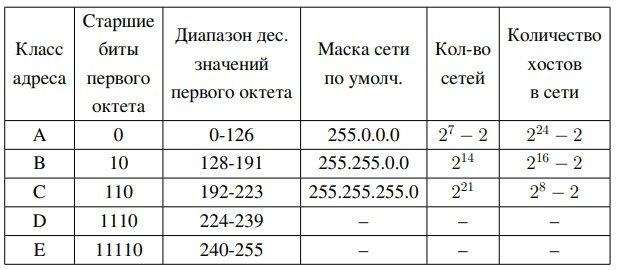
\includegraphics[width=1\textwidth]{1}
        \label{fig:image1}
    \end{figure}

\end{enumerate}

\section{Определение частей IP-адресов}

    Побитовое AND между маской и адресом даст нам сетевой адрес, побитовое OR между адресом и инвертированной маской даст нам широковещательный адрес

\begin{enumerate}
    \item Заполните таблицу:
    
    \begin{figure}[H]
        \centering      %размер рисунка       здесь находится название файла рисунка, без указания формата
        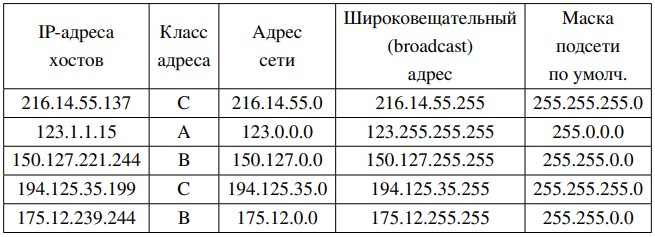
\includegraphics[width=1\textwidth]{2}
        \label{fig:image1}
    \end{figure}

    \item Дан IP-адрес 142.226.0.15
    \begin{enumerate}
        \item Чему равен двоичный эквивалент второго октета? 
        
        Ответ: 1110 0010
        \item Какому классу принадлежит этот адрес? 
        
        Ответ: B
        \item Чему равен адрес сети, в которой находится хост с этим адресом? 
        
        Ответ: 142.226.0.0
        \item Является ли этот адрес хоста допустимым в классической схеме адресации? 
        
        Ответ: нет, не является
        \item Почему да или почему нет? 
        
        Ответ: потому что адрес хоста состоит из октетов, содержащих только нули
    \end{enumerate}
\end{enumerate}

\section{IP-адреса хостов допустимые в коммерческих сетях}

    \begin{figure}[H]
        \centering      %размер рисунка       здесь находится название файла рисунка, без указания формата
        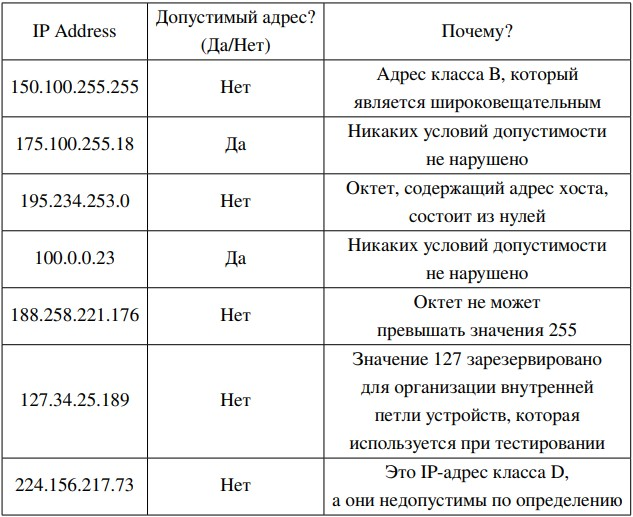
\includegraphics[width=1\textwidth]{3}
        \label{fig:image1}
    \end{figure}

\newpage
\section{Доставка пакетов по заданному IP-адресу}

    Если отправителем пакета является компьютер А, каким компьютерам из представленных на рисунке будет доставлен пакет с адресом.

    \begin{figure}[H]
        \centering
        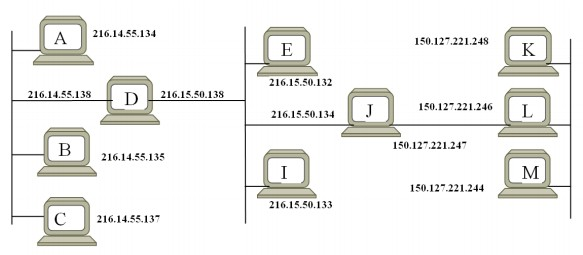
\includegraphics[width=1\textwidth]{4}
        \caption{Компьютерная сеть}
        \label{fig:img1}
    \end{figure}

\begin{enumerate}
    \item 0.0.0.0 
    
    Ответ: A
    \item 0.0.0.138 
    
    Ответ: D
    \item 255.255.255.255 
    
    Ответ: A, B, C, D, E, I, J, K, L, M
    \item 150.127.255.255 
    
    Ответ: K, L, M

\end{enumerate}

\section{Адресное пространство IPv4}
    \begin{enumerate}
        \item Укажите сколько сетей класса A и класса C доступно в схеме нумерации IPv4.
        
        Ответ: $2^7 - 2 + 2^{21}$ = 2097278
        \item Сколько хостов можно адресовать в каждой сети класса A и класса C в IPv4.
        
        Ответ: $2^{24} - 2 + 2^8 - 2$ = 16777468

        \item Сколько всего хостов можно разместить во всех сетях класса А и класса С.
        
        Ответ: количество хостов класса A во всех сетях класса A + количество хостов класса C во всех сетях класса C = 2113928964 + 532676608 = 2646605572

        \item Под размером адресного пространства понимается количество объектов, которым могут быть назначены адреса в рамках заданных правил. Поскольку в IPv4
        адрес это 32-битное двоичное число, то размер этого адресного пространства $2^{32}$. Какую часть этого пространства занимают адреса классов А, B, C и D.

        Ответ: $2^{32} - 2^4$ = 4294967280
        
    \end{enumerate}

\section{Вопросы для самопроверки}
    \begin{enumerate}
        \item Что такое IP адрес и для чего он используется?
        
        Ответ: IP-адрес — уникальный сетевой адрес узла в компьютерной сети, построенной на основе протокола IP. IP-адреса используют для однозначной
        идентификации отдельных сетей и хостов (персональных и специализированных компьютеров) в сетях при обеспечении связи между ними.

        \item Сколько классов IP адресов было определено при разработке протокола IPv4?
        
        Ответ: 5

        \item Что является критерием принадлежности IP адреса тому или иному классу?
        
        Ответ: В качестве критерия принадлежности IP адреса к тому или иному классу используют значение старших битов первого откета адреса.

        \item Из каких двух частей состоит IP адрес?

        Ответ: В базовом представлении IP-адрес состоит из двух частей - адреса сети и адреса хоста.
        
        \item Всегда ли IP адрес включает в себя и адрес сети и адрес узла в этой сети?
        
        Ответ: Если часть адреса - адрес хоста содержит все 0, то это адрес самой сети без указания адреса хоста. Если адрес хоста содержит все 1, 
        то это широковещательный адрес в заданной сети (это означает, что пакет адресован всем хостам).

        \item В каком случае IP адрес является адресом всей сети а не отдельного узла сети?
        
        Ответ: Если в поле номера сети стоят только нули, то по умолчанию считается, что узел назначения принадлежит той же самой сети, что и узел, который
        отправил пакет.

        \item В каком случае IP адрес предписывает сетевым устройствам адресовать сообщение всем узлам некоторой сети?
        
        Ответ: Если в поле адреса назначения стоят сплошные 1, то пакет, имеющий такой адрес рассылается всем узлам сети с заданным номером. Такая рассылка
        называется широковещательным сообщением

        \item Что такое маска сети?

        Ответ: Маской сети называется битовая маска, определяющая, какая часть IPадреса является адресом сети, а какая определяет адрес узла в этой сети.
        Например, узел с IP-адресом 12.34.56.78 и маской сети 255.255.255.0 находится в сети 12.34.56.0.

       \item Какие IP адреса можно использовать без получения разрешения у администрации Internet?
        
       Ответ:

            \begin{enumerate}
                \item 10.0.0.0 - 10.255.255.255
                \item 172.16.0.0 - 172.31.255.255
                \item 192.168.0.0 - 192.168.255.255
                \item 169.254.0.0 - 169.254.255.255
            \end{enumerate}

       \item Почему выделение специальных диапазонов сетевых адресов, используемых только внутри закрытых сетей, экономит адресное пространство для
       Internet?
       
       Выделение отдельных диапазонов сетевых адресов для закрытых сетей экономит адресное пространство для Internet тем, что часть адресов, которая 
       могла бы быть занята этими закрытыми сетями, никак не связанными со всемирной сетью, может использоваться для реализации открытых сетей, и таким 
       образом повышается эффективность использования адресного пространства.
       
    \end{enumerate}


\end{document}
